\subsection{Motivation}
In order to try to confirm that the game variants generated had the intended effects on gameplay, we initially generated AI agents to play the games. We would then log the score, velocity, and missile count of each of the agents over the course of multiple runs, and use these results to try to try to quantify the effects of the variations in the game.

\subsection{Methodology}


For the purpose of testing the different variations of the game, 4 agents were used: MCTS with 40ms thinking time, MCTS with 20ms thinking time, RotateAndShoot and EmptyAI.
The assumption we made was that the 40ms MCTS would perform a lot better than the 20ms MCTS and that both would greatly overperform compared to RotateAndShoot and EmptyAI. The MCTS agents were also expected to perform admirably against human players.

During the IGGI Essex GD2 training courses, MCTS was found to be the best technique for this sort of game by far with 66 wins and only 4 losses in a round robin tournament between 7 algorithms playing against each other in a game of Battle Asteroids. The next best AI managed 56 wins and 14 losses, but employed a lot of knowledge relevant to that simpler variation of Battle Asteroids. As a result of these findings, MCTS was picked as the only AI to challenge the game and the human players.

Both MCTS agents make use of a rollout depth of 16 and 3 macro actions. The use of macro actions allows the search space to grow more in a helpful manner, thus finding better moves overall. ({Powley, E.J. and Whitehouse, D. and Cowling, P.I.}) As mentioned previously, the only difference between them is the halved time to think the second agent has. This should, in theory, result in a worse performing agent, at least compared to the other agent.

RotateAndShoot employs a very simple behaviour: it is always rotating in one direction and it is always shooting. During the IGGI Essex GD2 trials, RotateAndShoot failed to beat any of the other AI implementations, but often did score positively regardless of eventual loss. Its inclusion helped demonstrate any clear differences in missile avoidance between the various game types and agents.

EmptyAI does nothing and is there to showcase the MCTS agents’ attempts at collecting as many points as possible, with minimal / no resistance from the opponent.

Following the IGGI Essex GD2 example, a round robin tournament was decided to test the 4 different agents competing against each other in all 3 variations of the game. This had two aims: to assess automated playability of each game variation, as well as understand how scoring affected changes between games. If the MCTS agents successfully collect a fair number of powerups and manage to hit the opponents often enough, while also avoiding asteroids (where applicable) and avoid being hit by the other player, one can assume the game is in a playable state. This must also be confirmed (or infirmed) by human testing.

The tournament consisted of each agent playing each other agent 30 times. This resulted in 180 matchups. Information about score over time, velocity over time and missiles left over time was stored (see figure X).

\subsection{Results}

Results of the tournament on the first variation of the game (asteroids that split) show the 40ms MCTS agent behaving best. This is as predicted, as the tree the algorithm can expand is much greater than the one the 20ms MCTS agent can create, thus being able to choose better moves every tick. 

This also proves the game will favour more skillful players to random ones and reward better play. The game is challenging enough that the weaker MCTS agent can still win, just not often enough compared to the one given more thinking time.

\begin{figure}
	\caption{AI results over the game without}
	\begin{tabular}{p{7.5em} | p{4.5em} p{4.5em} p{4.5em} p{4.5em}}
		&
			Empty Controller &
			Rotate and Shoot &
			MCTS (20ns) &
			MCTS (40ms) \\ \hline
		Empty Controller &
			-&
			0\% &
			3\% &
			0\% \\
		Rotate and Shoot &
			1000\% &
			-&
			3\% &
			3\% \\ 
		MCTS (20ns) &
			97\% &
			97\% &
			-&
			30\% \\
		MCTS (40ns) &
			100\% &
			97\% &
			70\% &
			-\\
	\end{tabular}
\end{figure}

\begin{figure}
	\caption{AI results over the game with simple asteroids}
	\begin{tabular}{p{7.5em} | p{4.5em} p{4.5em} p{4.5em} p{4.5em}}
		&
			Empty Controller &
			Rotate and Shoot &
			MCTS (20ms) &
			MCTS (40ms) \\ \hline
		Empty Controller &
			-&
			0\% &
			0\% &
			0\% \\
		Rotate and Shoot &
			100\% &
			-&
			20\% &
			6\% \\ 
		MCTS (20ms) &
			100\% &
			80\% &
			-&
			57\% \\
		MCTS (40ms) &
			100\% &
			93\% &
			44\% &
			-\\
	\end{tabular}
\end{figure}

\begin{figure}
	\caption{AI results over the game with splitting asteroids}
	\begin{tabular}{p{7.5em} | p{4.5em} p{4.5em} p{4.5em} p{4.5em}}
		&
			Empty Controller &
			Rotate and Shoot &
			MCTS (20ms) &
			MCTS (40ms) \\ \hline
		Empty Controller &
			-&
			3\% &
			0\% &	
			0\% \\
		Rotate and Shoot &
			97\% &
			-&
			3\% &
			0\% \\ 
		MCTS (20ms) &
			100\% &
			97\% &
			-&
			30\% \\
		MCTS (40ms) &
			100\% &
			100\% &
			70\% &
			-\\
	\end{tabular}
\end{figure}

\begin{figure}
	\caption{Average metrics for AI players over the game without asteroids}
	\center
	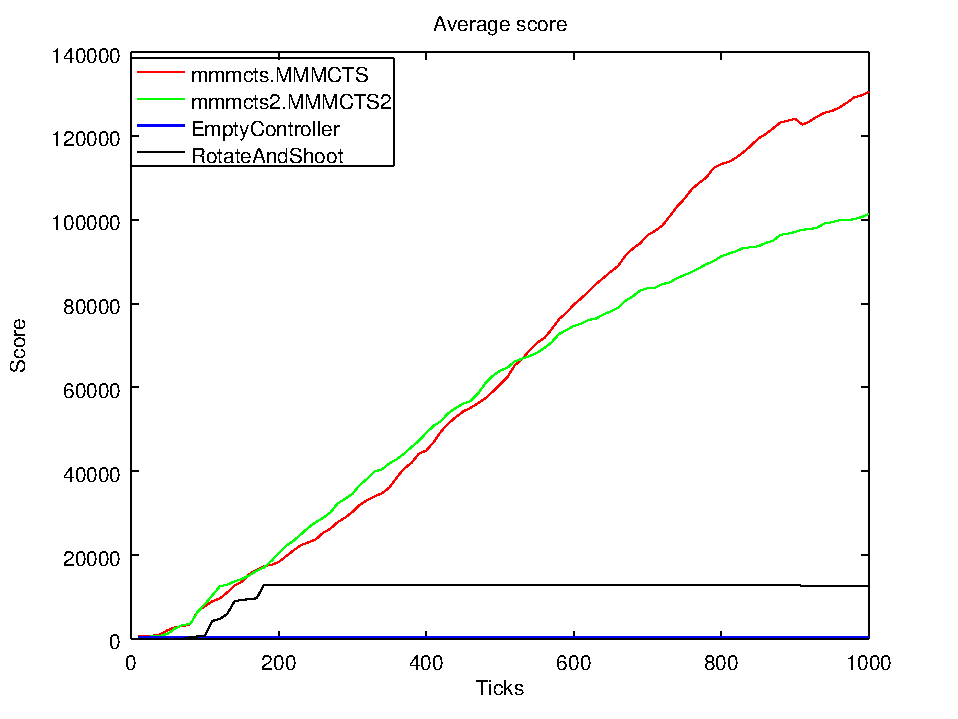
\includegraphics[scale=0.25]{resources/score_2.pdf}
	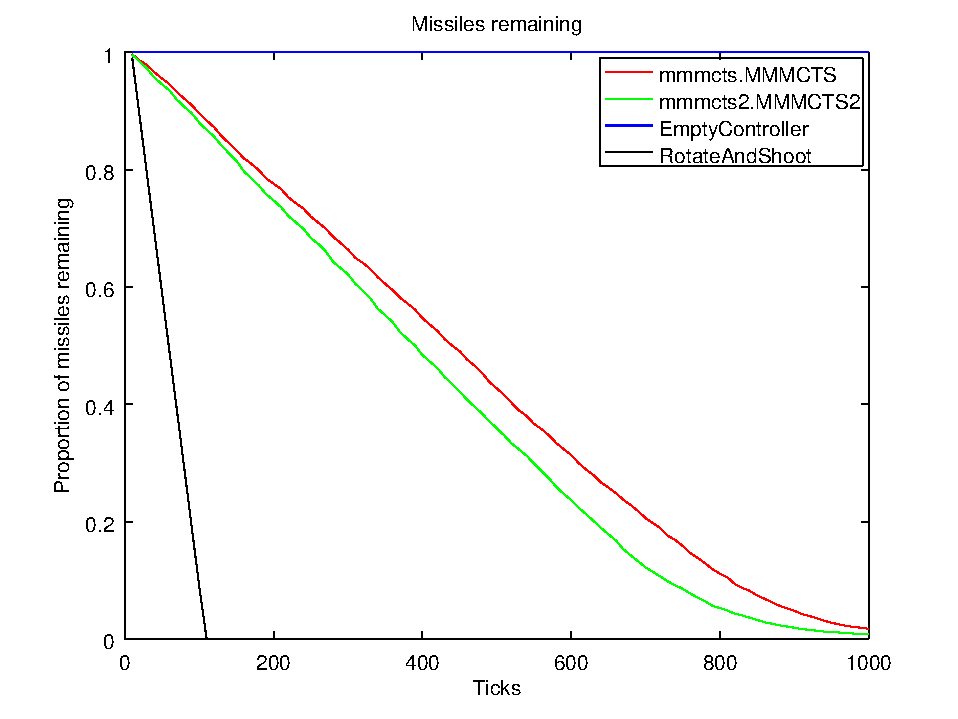
\includegraphics[scale=0.25]{resources/missiles_2.pdf}
\end{figure}

\begin{figure}
	\caption{Average metrics for AI players over the game with simple asteroids}
	\center
	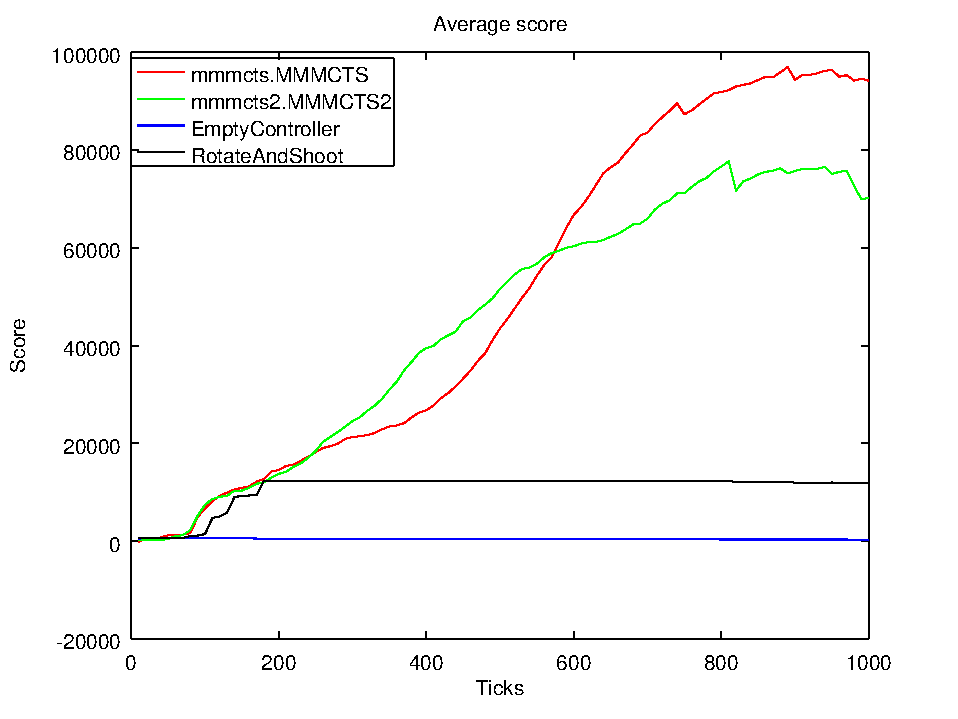
\includegraphics[scale=0.25]{resources/score_1.pdf}
	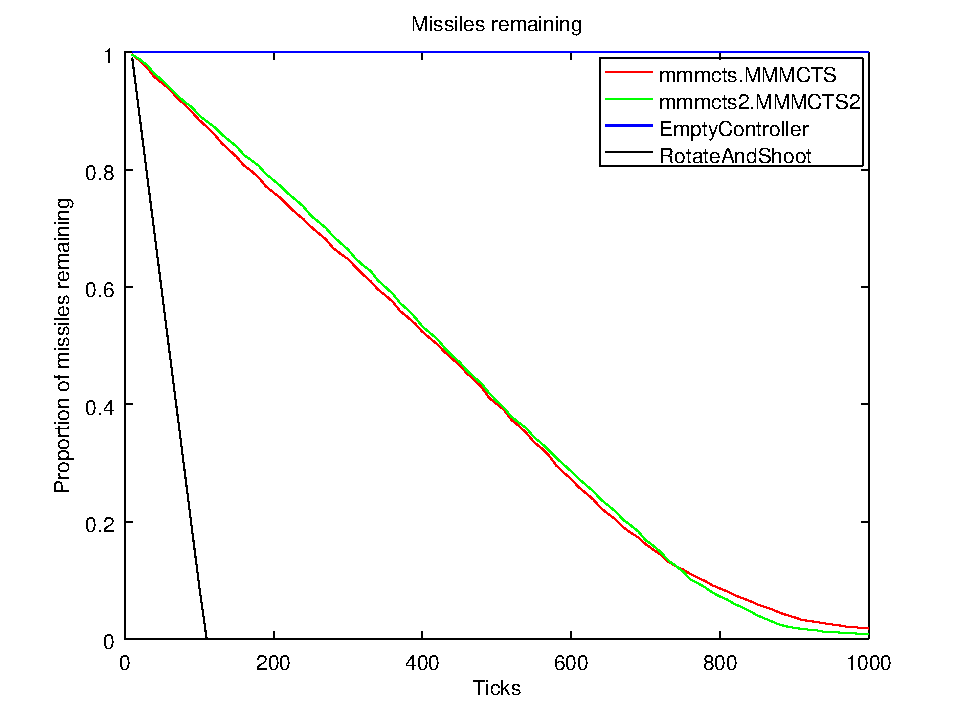
\includegraphics[scale=0.25]{resources/missiles_1.pdf}
\end{figure}

\begin{figure}
	\caption{Average metrics for AI players over the game with splitting asteroids}
	\center
	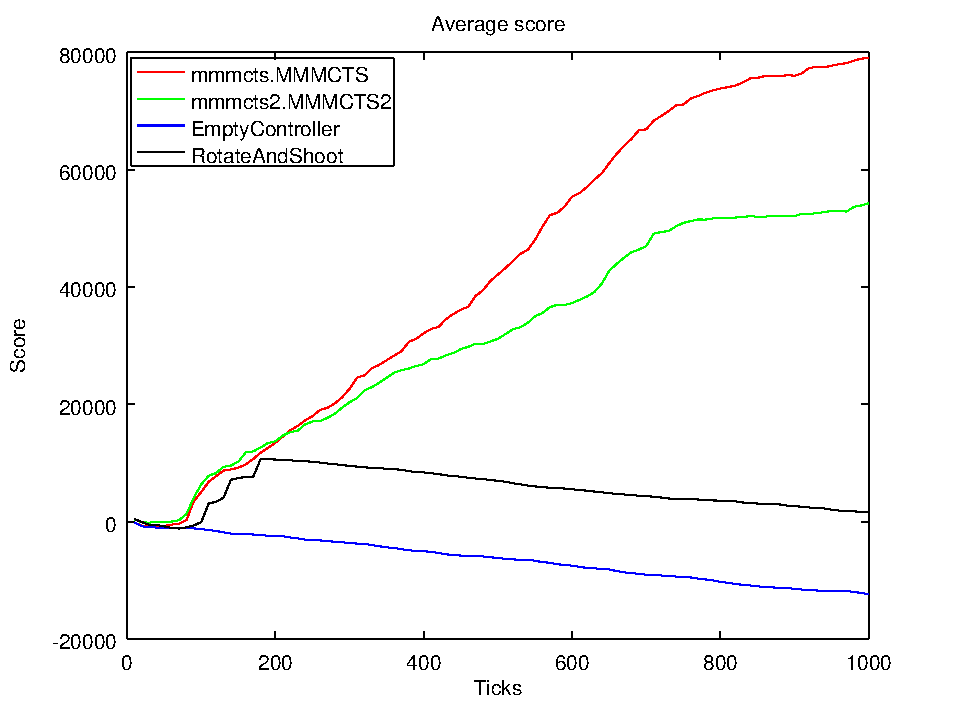
\includegraphics[scale=0.25]{resources/score_0.pdf}
	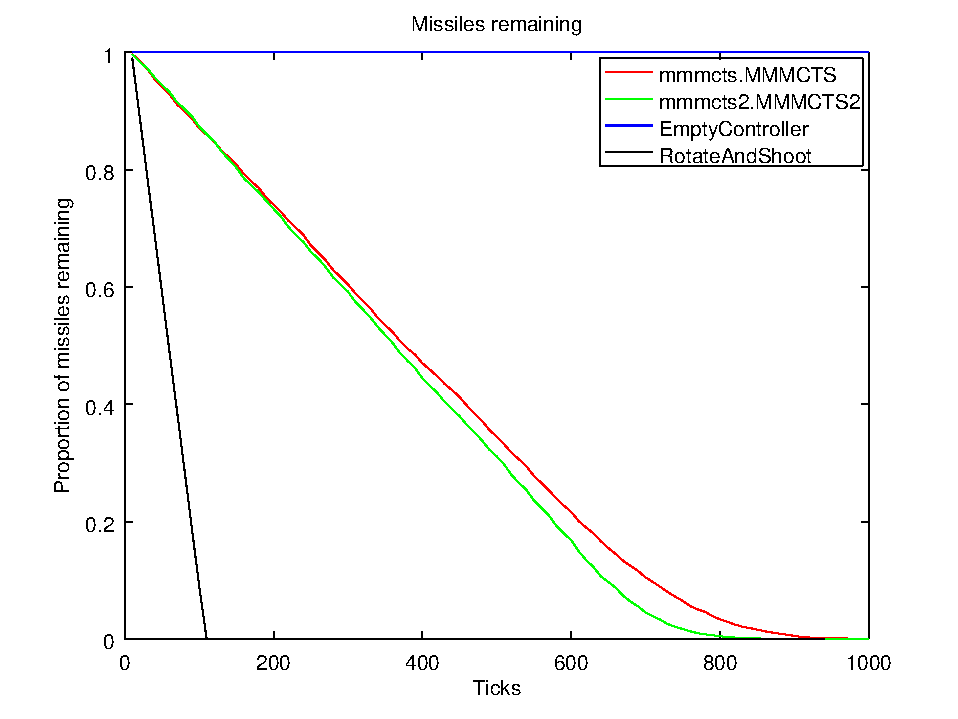
\includegraphics[scale=0.25]{resources/missiles_0.pdf}
\end{figure}